\subsection{Front-end module architecture}
This section shows how the Front-end\textsubscript{G} module of EmporioLambda works. \\The Front-end\textsubscript{G} module can be summarized in 4 primary parts:
\begin{itemize}
\item \textbf{data pre-fetching:} managed with Next.js\textsubscript{G};
\item \textbf{components:} managed with React;
\item \textbf{services:} functions that communicate with the Back-end\textsubscript{G} module;
\item \textbf{types:} classes and data types used.
\end{itemize} 
The image below shows how these parts communicate with each other:
\begin{figure}[H]
\centering
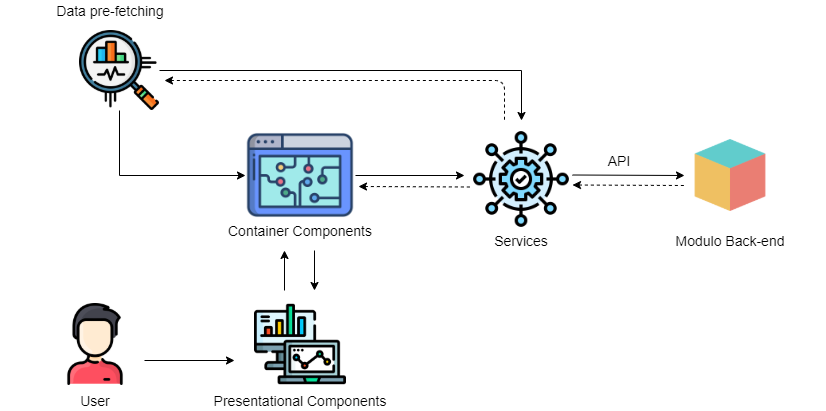
\includegraphics[scale=0.70]{res/Architettura/Frontend/img/general_frontend}\\
\caption{Front-end\textsubscript{G} module general scheme}
\end{figure}
\newpage
Here's also a package diagram of the Front-end module:
\begin{figure}[H]
\centering
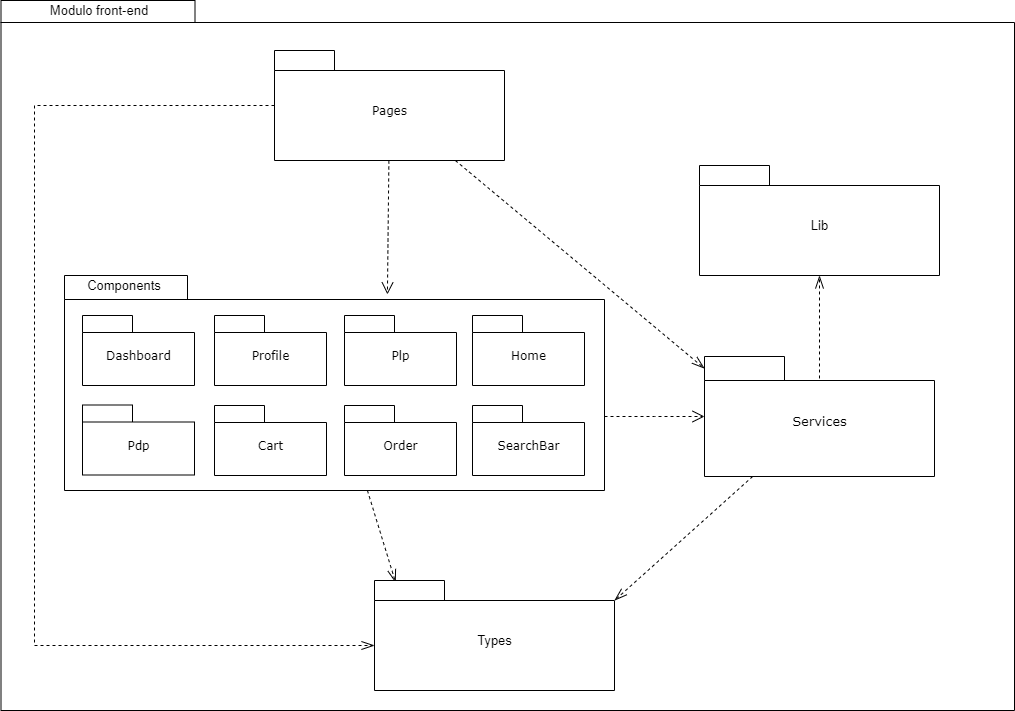
\includegraphics[scale=0.40]{res/Architettura/Frontend/img/package_frontend}\\
\caption{Front-end\textsubscript{G} module package\textsubscript{G} diagram}
\end{figure}

\textbf{lib}: contains support functions to standardize the calls to our Back-end module\textsubscript{G}.\\
 The rest of the packages will be explained in the next sections.

\newpage
In the following sequence diagram, representing the insertion of an item in the cart, is possible to see how the different parts of the Front-end module work:
\begin{figure}[H]
\centering
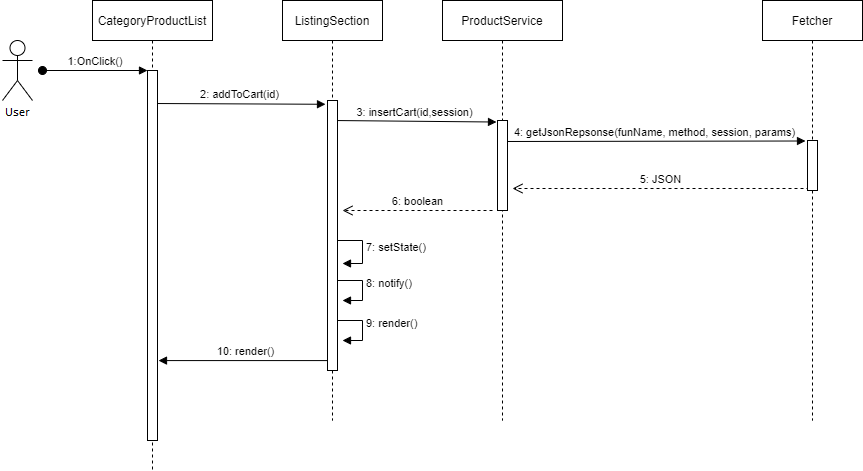
\includegraphics[scale=0.70]{res/Architettura/Frontend/img/sequence_frontend_insertCart}\\
\caption{Front-end\textsubscript{G} module insert of an item in cart sequence diagram}
\end{figure}


